\chapter{State of the art}
This chapter will go through relevant articles and already known knowledge on the subject of mixed criticality systems. It will also explain the EMC2DP.

\section{Mixed criticality systems}
%SotA regarding MCS.
A MCS is achieved by letting applications of different criticality share resources. These resources could be the processor, memory, peripherals, input/output ports etc. The most explored area is sharing the CPU between multiple criticality levels \cite{burns2016}. The benefit of combining previously distributed systems is higher resource efficiency, which leads to economical benefits.\\

%The term Mixed Criticality had been used before 2007 to address issues of non-interference in non-federated architectures such as IMA [190];

\subsection{Economical benefits of MCS}
%Lower production cost, higher design cost?
Potential benefits with pursuing MCS as opposed to distributed systems are reduced physical space required, reduced weight, reduced heat generation, reduced power consumption and reduced production costs~\cite{burns2016}. This would all ultimately lead to economical benefits.\\

Potential downsides are increased complexity which could lead to higher system design costs. Building applications on the same platform to share resources could require engineering teams to work more closely together, potentially leading to administrative difficulties and costs. This needs to be investigated and could vary from industry to industry. To combat the potential downsides, the EMC\textsuperscript{2} project aims at creating platforms for easier development of MCS.\\ %TODO: källa eller ändra wording

The EMC\textsuperscript{2} project lists several goals \cite{website:emc2goals}:
\begin{itemize}
\item Reduce the cost of the system design by 15\%
\item Reduce the effort and time required for re-validation and re-certification of systems after making changes by 15\%
\item Manage a complexity increase of 25\% with 10\% effort reduction
\item Achieve cross-sectorial reusability of Embedded Systems devices and architecture platforms that will be developed using the ARTEMIS JU results.
\end{itemize}

\subsection{Sharing processor}
%A lot of work has been done regarding processor scheduling in MCS
%TODO: Wording
To deal with many different tasks needing processor time, different schedulers can be used to appropriately distribute processor time among the tasks.

\subsubsection{Conventional scheduling}
Fixed priority
Deadline monotonic
Rate monotonic
Earliest deadline first
Round robin

\subsubsection{Mixed criticality scheduling}
The area of sharing the processor in MCS was first explored by Steve Vestal~\cite{vestal2007} in 2007. His paper showed that neither Rate Monotonic (RM) nor Deadline Monotonic (DM) priority assignment was optimal for MCS; however Audsley’s optimal priority assignment algorithm \cite{audsley2001} was found to be applicable.\\ %TODO: Wording

In 2008 Baruah and Vestal~\cite{baruah2008} showed that EDF (Earliest Deadline First) does not dominate FP when criticality levels are introduced, and that there are feasible systems that cannot be scheduled by EDF.\\

One MCS scheduling algorithm is Criticality Monotonic Priority Ordering (CrMPO). Tasks are assigned priorities first according to criticality (highest criticality first) and then according to deadline (shortest deadline first). Static Mixed Criticality with no run-time monitoring (SMC-NO) is the scheduler that was Vestal's original approach~\cite{vestal2007}. Another scheduler is SMC with run-time monitoring (abbreviated only as SMC). Yet another scheduling algorithm is Adaptive Mixed Criticality (AMC), described Baruah, Burns and Davis~\cite{baruah2011}: "To summarise the main difference between SMC and AMC, in SMC any LO-critical task is descheduled if it executes for more than C(LO). While in AMC, all LO-critical tasks are descheduled if any job (from any task) executes for more than C(LO). If a HI-critical job executes for more than C(LO) (but no greater than C(HI)) then, under SMC, LO-critical tasks continue to execute but may miss their deadlines; but under AMC they stop executing."\\

To evaluate the performance of the different scheduling algorithms Baruah, Burns and Davis~\cite{baruah2011} tested the scheduling algorithms AMC, SMC and CrMPO for scheduling sporadic tasks of a taskset of 20 tasks where on average 50\% where of high criticality and 50\% where of low criticality. The tasks of high criticality where allowed an execution time that was twice its low criticality execution time. The comparison of the performance of the schedulers can be seen in Figure~\ref{fig:schedulers}. In the graph the UB-H\&L line bounds the maximum possible number of schedulable task sets.

%"This figure plots the percentage of task sets generated that were deemed schedulable for a system of 20 tasks, with on average 50\% of those tasks having high criticality and each task having a high criticality execution time that is twice its low criticality execution time. The compared approaches are (from least effective to most effective): CrMPO which assigned priorities in criticality order, SMC-NO (static  mixed criticality with no run-time  monitoring) which  is  Vestal’s  original approach, SMC which is an adaptation of Vestal’s approach in which LO-criticality tasks are monitored at run-time and are prevented from executing for more than C(LO), and AMC-rtb and AMC-max which are the two methods introduced in the previous paragraph (AMC for adaptive mixed criticality). In the graph the UB-H\&L line bounds the maximum possible number of schedulable task sets. It serves to illustrate the quality of the AMC-max approach."~\cite{burns2016}

\begin{figure}[H]
\centering
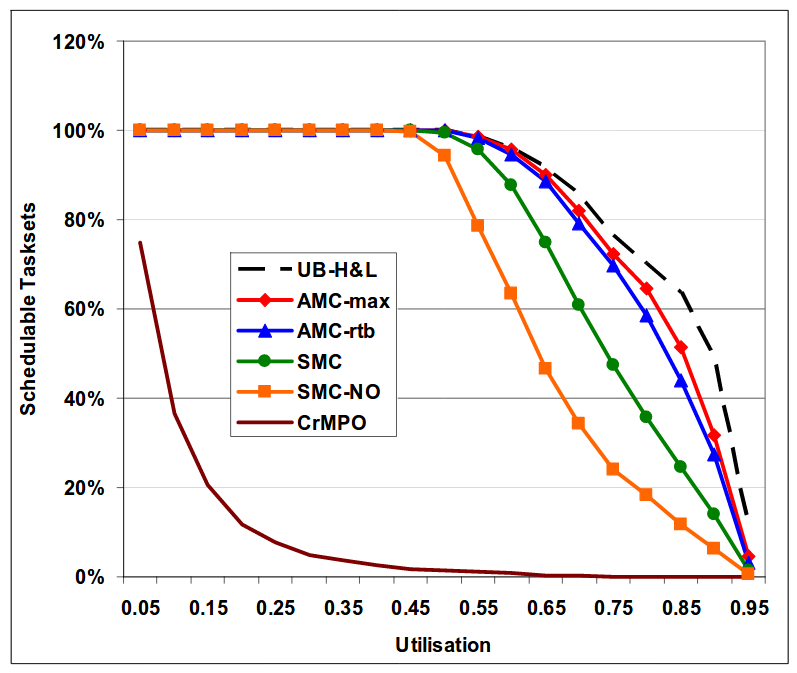
\includegraphics[width=\textwidth]{./img/literature_schedulers.png}
\caption{Percentage of schedulable tasks.~\cite{baruah2011}}\label{fig:schedulers}
\end{figure}

For a more complete review of work done on MCSs with a shared processor, see the paper by Burns~\cite{burns2016}.

%\subsection{Different criticality on different processors}


%\subsection{Sharing memory}
%http://pertsserver.cs.uiuc.edu/~mcaccamo/papers/euromicro12.pdf

\section{Standards}
%Different standards to regulate and ensure safety
Safety practices are becoming more regulated as industries adopt a standardized set of practices for designing and testing products. %TODO: expand, wording

\subsection{IEC 61508}
IEC 61508~\cite{IEC61508} is intended to be a basic functional safety standard for electrical and electronic systems applicable to all kinds of industry. It defines four different safety integrity levels, SIL~1 being the least dependable up to SIL~4 which is the most dependable level.

\subsection{ISO 26262}
ISO 26262~\cite{ISO26262} addresses the needs for an automotive-specific international standard that focuses on safety critical components. ISO 26262 is a derivative of IEC 61508.

\subsubsection{ASILs}
%ASIL QM (quality management) relates to the lowest (no) hazard, and ASIL
ISO 26262 describes five different Automotive Safety Integrity Levels (ASIL) relating to hazard and risk. Ranked from lowest (no) hazard to highest hazard, these levels are: QM, A, B, C and D. A function is assigned an ASIL depending on the severity if the function fails, the probability that the function fails and the controllability of the function, see table~\ref{table:ASIL}.

\begin{table}[H]
\centering
\begin{tabular}{|c|c|c|c|c|}
\hline
\multirow{2}{*}{\textbf{Severity}} &\multirow{2}{*}{\textbf{Probability}} &\multicolumn{3}{|c|}{\textbf{Controllability}} \\ \cline{3-5}
 & &C1 &C2 &C3 \\ \hline
\multirow{4}{*}{S1} & E1 & QM & QM & QM \\ \cline{2-5}
 & E2 & QM & QM & QM \\ \cline{2-5}
 & E3 & QM & QM & A \\ \cline{2-5}
 & E4 & QM & A & B \\ \hline
\multirow{4}{*}{S2} & E1 & QM & QM & QM \\ \cline{2-5}
 & E2 & QM & QM & A \\ \cline{2-5}
 & E3 & QM & A & B \\ \cline{2-5}
 & E4 & A & B & C \\ \hline
\multirow{4}{*}{S3} & E1 & QM & QM & A \\ \cline{2-5}
 & E2 & QM & A & B \\ \cline{2-5}
 & E3 & A & B & C \\ \cline{2-5}
 & E4 & B & C & D \\ \hline
\end{tabular}
\caption{ASIL as a function of severity, probability and controllability.}
\label{table:ASIL}
\end{table}

The various integrity levels can be translated into integers (ASIL $QM = 0$; $A = 1$; $B = 2$; $C = 3$ and $D = 4$). If a hazard requires several components to fail, the added ASIL of these components is used to determine if there is an violation, assuming the components faults are statistically independent of each other. For example, a safety level ASIL B can be met by two independent components which each individually only meet ASIL A (and thus effectively $A + A = B$).~\cite{azevedo2014} \\ %TODO: semi Wording

The different ASILs can relate to cost according to various cost heuristics, see table~\ref{table:cost_heuritics}. %TODO: Expand, wording

\begin{table}[H]
\centering
\begin{tabular}{|c|c|c|c|c|c|}
\hline
\textbf{Cost Heuristic} & \textbf{QM} & \textbf{A} & \textbf{B} & \textbf{C} & \textbf{D} \\ \hline
Linear & 0 & 10 & 20 & 30 & 40 \\ \hline
Logarithmic & 0 & 10 & 100 & 1000 & 10000 \\ \hline
Experimental-I~\cite{azevedo2014} & 0 & 10 & 20 & 40 & 50 \\ \hline
Experimental-II~\cite{azevedo2014} & 0 & 20 & 30 & 45 & 55 \\ \hline
\end{tabular}
\caption{ASIL cost heuristics.}
\label{table:cost_heuritics}
\end{table}


\subsubsection{Freedom from interference}
%TODO: Källa, utveckla, wording
In ISO 26262, Part 1, Definition 1.49, freedom from interference is defined as: Absence of cascading failures between two or more elements that could lead to the violation of a safety requirement. A cascading failure is defined as = "failure of an element of an item causing another element or elements of the same item to fail" (ISO 26262, Part 1, Definition 1.13), and an element is defined as: "system or part of a system including components, hardware, software, hardware parts, and software units" (ISO 26262, Part 1, Definition 1.32)

\subsection{AUTOSAR}
%TODO: Wording
"AUTOSAR (AUTomotive Open System ARchitecture) is a international development partnership of automotive interested parties founded in 2003. It pursues the objective of creating and establishing an open and standardized software architecture for automotive electronic control units (ECUs) excluding infotainment. Goals include the scalability to different vehicle and platform variants, transferability of software, the consideration of availability and safety requirements, a collaboration between various partners, sustainable utilization of natural resources, maintainability throughout the whole "Product Life Cycle"."~\cite{website:autosar}\\

The AUTOSAR Architecture distinguishes on the highest abstraction level between three software layers: Application, Runtime Environment (RTE) and Basic Software (BSW) which run on a Microcontroller.~\cite{website:autosar} See figure \ref{fig:autosar}.
\begin{itemize}
\item The application software layer is mostly hardware independent.
\item The RTE represents the full interface for applications.
\item The BSW is divided in three major layers and Complex Drivers: Services, ECU Abstraction and Microcontroller Abstraction. Services are divided furthermore into functional groups representing the infrastructure for System, Memory and Communication Services.
\end{itemize}

\begin{figure}[H]
\centering
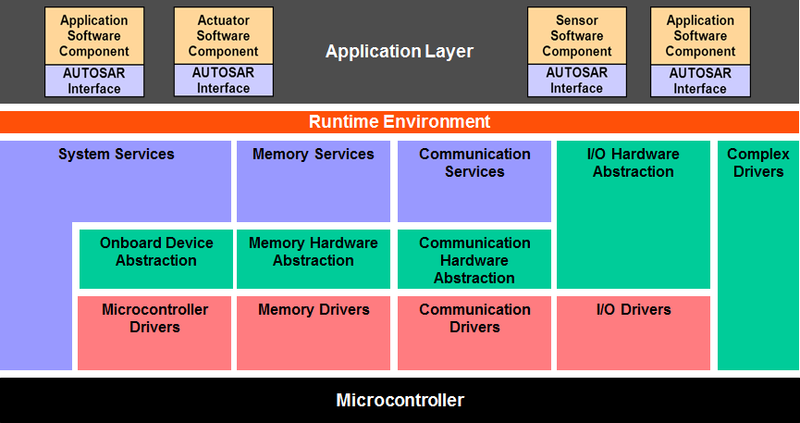
\includegraphics[width=\textwidth]{./img/literature_autosar.png}
\caption{AUTOSAR.~\cite{website:autosar}}\label{fig:autosar}
\end{figure}

\section{Mixed criticality platform solutions}
%Literature study about platfrom solutions for MCS

\section{Platooning}
%TODO: wording
Vehicle platooning can be described as a chain of vehicles traveling at a given intermediate distance and velocity. The primary objective for each vehicle with respect to safety is to maintain its distance to the preceding vehicle in the platoon. A platoon of N vehicles is often modeled in the literature as a set of moving point masses

\subsection{Benefits of platooning}
In Alam, Gattami, and Johansson (2010) it has been shown that there is a 4.7–7.7\% fuel reduction potential in HDV platooning.